\documentclass{article}
\usepackage[margin=1in]{geometry}
\usepackage{amsmath,amsthm,amssymb}
\usepackage{bbm,enumerate,mathtools}
\usepackage{tikz,pgfplots}
\usepackage{chessboard}
\usepackage[hidelinks]{hyperref}
\usepackage{multicol} % Problem 35

\newenvironment{question}{\begin{trivlist}\item[\textbf{Question.}]}{\end{trivlist}}
\newenvironment{note}{\begin{trivlist}\item[\textbf{Note.}]}{\end{trivlist}}
\newenvironment{references}{\begin{trivlist}\item[\textbf{References.}]}{\end{trivlist}}
\newenvironment{related}{\begin{trivlist}\item[\textbf{Related.}]\end{trivlist}\begin{enumerate}}{\end{enumerate}}


\begin{document}
\rating{2}{2}
In the game (tic-tac-toe)$^2$, each square is itself a smaller tic-tac-toe game;
of course, one could imagine (tic-tac-toe)$^3$, where each of the squares in
the smaller tic-tac-toe boards are themselves tic-tac-toe boards and so on.
We're interested in counting (an abstraction of) the number of boards in this game,
where two boards are considered the same if one is a rotation/reflection of
another, or if any of the iterated games is a rotation/reflection of another,
and so on.

In the simplest version, the boards are $2 \times 2$ and every square is
filled in with an ``X'' or an ``O'', in perhaps unequal numbers.

\begin{figure}[ht!]
  \centering
  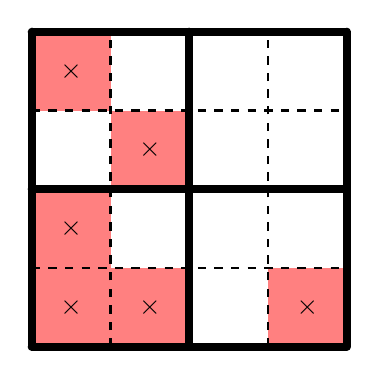
\begin{tikzpicture}
    \foreach \x/\y in {0/0, 1/0, 0/1, 0/3, 1/2, 3/0} {
      \fill[red!50] (\x,\y) rectangle (\x+1,\y+1);
      \node at (\x+0.5,\y+0.5) {$\times$};
    }

    \draw[thick, dashed]                        (0,0) grid (4,4);
    \draw[line width=3, line cap=round, step=2] (0,0) grid (4,4);
  \end{tikzpicture}
  ~
  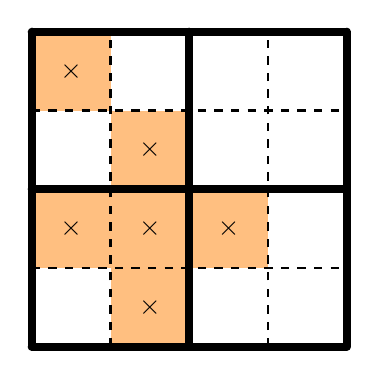
\begin{tikzpicture}
    \foreach \x/\y in {1/1, 1/0, 0/1, 0/3, 1/2, 2/1} {
      \fill[orange!50] (\x,\y) rectangle (\x+1,\y+1);
      \node at (\x+0.5,\y+0.5) {$\times$};
    }

    \draw[thick, dashed]                        (0,0) grid (4,4);
    \draw[line width=3, line cap=round, step=2] (0,0) grid (4,4);
  \end{tikzpicture}
  ~
  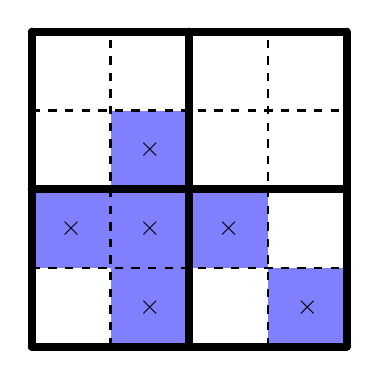
\begin{tikzpicture}
    \foreach \x/\y in {1/1, 1/0, 0/1, 3/0, 1/2, 2/1} {
      \fill[blue!50] (\x,\y) rectangle (\x+1,\y+1);
      \node at (\x+0.5,\y+0.5) {$\times$};
    }

    \draw[thick, dashed]                        (0,0) grid (4,4);
    \draw[line width=3, line cap=round, step=2] (0,0) grid (4,4);
  \end{tikzpicture}
  \caption{
    Three boards of depth $2$ that are equivalent up to dihedral
    actions of both the smaller and larger boards.
  }
\end{figure}

\begin{question}
  How many different boards of depth $n$ are there?
\end{question}

\begin{related}
  \item What if these are counted up to interchanging all ``Xs'' and ``Os''?
  \item What if done on nested $m \times m$ boards?
  \item What if the biggest board is $m_1 \times m_1$, the second level of
    boards are $m_2 \times m_2$, the $i$-th level of boards are
    $m_i \times m_i$ and so on?
  \item How does this work in higher dimensions? On other grids?
  On polygons on the vertices of polygons (on the vertices of polygons)?
\end{related}

\begin{note}
  It appears that the group that acts on an ordinary board is $D_8$.
  The group that acts on a depth-2 board is $D_8 \wr D_8$, a depth-3 board is
  $(D_8 \wr D_8) \wr D_8 $ and so on.
\end{note}
\begin{references}
  \item Problems 31, 61, 79, 86, and 91.
  \item \href{https://en.wikipedia.org/wiki/Ultimate_tic-tac-toe}{Wikipedia, Ultimate tic-tac-toe}.
\end{references}
\end{document}
